\begin{section}{ACE}{Investigating the Origin of Clumps in the CGM using \\
    \hspace*{4cm} Hydrodynamical Simulations}{(Ann-Christine Vossberg, PhD)}
  \begin{minipage}{\linewidth}
    \begin{wrapfigure}{r}{0pt}
      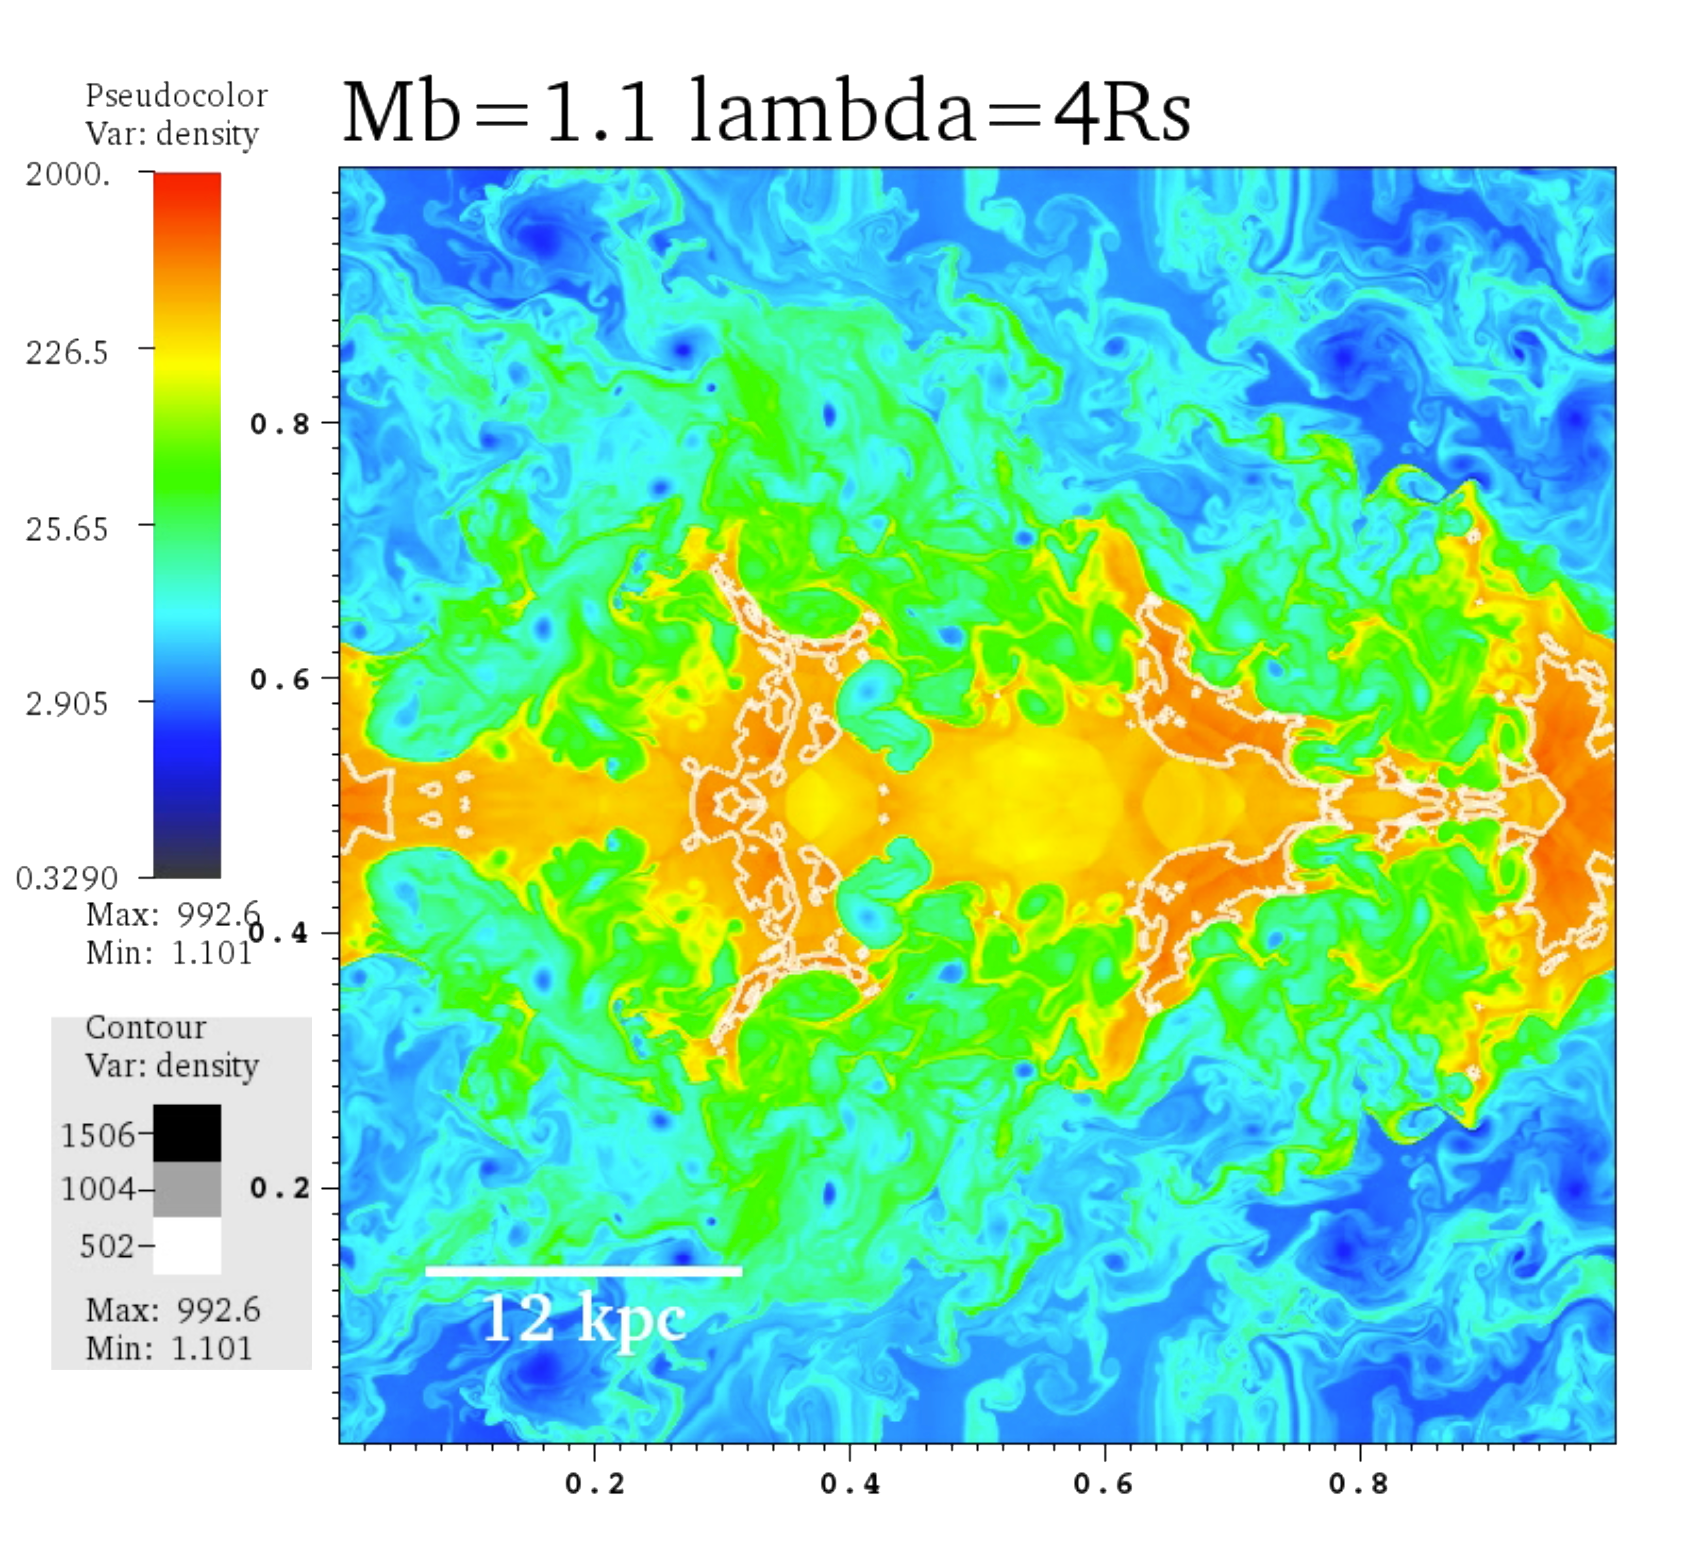
\includegraphics[height=13cm]{ACE/Ramses-2.png}
    \end{wrapfigure}
    \strut {\small In order to understand the dominant processes in accreting
      filamentary structures and the origin of their physical properties we use
      2D idealized high-resolution simulations (RAMSES). This allows us to
      investigate how different processes effect a filament, its evolution,
      morphology and its survival. Thermally unstable accreting filaments will
      not stay laminar but will be subject to KHI and an interplay of cooling
      and heating. We find that Kelvin-Helmholtz Instability (KHI) in the
      nonlinear regime may act as a trigger for forming clumps. Additionally KHI
      has the potential to destroy the filament under certain circumstances.
      These circumstances largely depend on the Mach-Number of the filament, the
      perturbation wavelength and the thickness of the interface between the
      halo and filament. When cooling is introduced the density distribution
      tail of the filament reaches ~14 times the initial filament density and
      consequently increases the Clumping factor. KHI coupled with radiative
      cooling may be one reason for the observed high Clumping factor in
      observations.}
  \end{minipage}
\end{section}